\chapter{Технологический раздел}

\section{Язык программирования}
В качестве языка программирований выбран язык высокого уровня JavaScript.

\section{Примеры кода}

\begin{lstlisting}[caption={Получение коэфициентов уравнений Колмагорова}]
function getKoefKolmagorof(matrix) {
    let result = [];
    for (let i = 0, n = matrix.length; i < n; ++i) {
		result[i] = [];

        for (let j = 0, m = matrix[i].length; j < m; ++j) {
            result[i][j] = 0;
        }
    }

    for (let i = 0, n = matrix.length; i < n; ++i) {
        for (let j = 0, m = matrix[i].length; j < m; ++j) {
        	if (i != j) {
            	result[i][i] -= matrix[i][j];
        	}
        }
    }

    for (let i = 0, n = matrix.length; i < n; ++i) {
        for (let j = 0, m = matrix[i].length; j < m; ++j) {
        	if (i != j) {
            	result[j][i] += matrix[i][j];
        	}
        }
    }

    return result;
}
\end{lstlisting}

\section{Взаимодейсвтие с пользователем}

Взаимодейсвтие с пользователем осуществляется через html страницы, открытые в браузере. В пользовательском интерфесе используются динамические таблицы \cite{softtime-table}. 

\begin{figure}
  \centering
  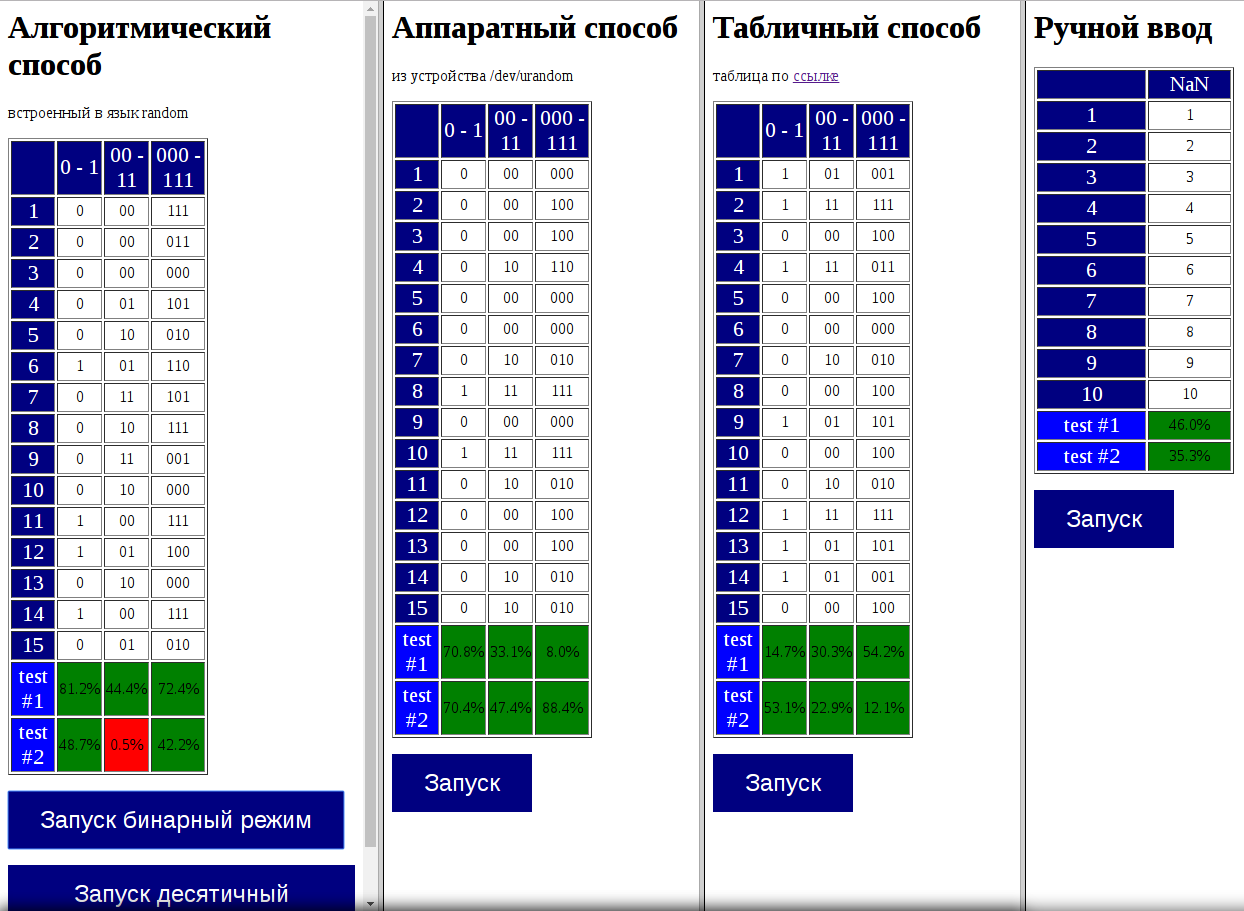
\includegraphics{screen1.png}
  \caption{Пример работы программы}
\end{figure}
